\documentclass[12pt, twoside]{book}
%\documentclass[12pt, oneside]{book}  % jednostranna tlac
\usepackage[a4paper,top=2.5cm,bottom=2.5cm,left=3.5cm,right=2cm]{geometry}
\usepackage[utf8]{inputenc}
\usepackage[T1]{fontenc}
\usepackage{graphicx}
\usepackage{url}
\usepackage[hidelinks,breaklinks]{hyperref}
\usepackage[slovak]{babel} % vypnite pre prace v anglictine
\linespread{1.25} % hodnota 1.25 by mala zodpovedat 1.5 riadkovaniu

\usepackage{caption}
\usepackage{subcaption}
\usepackage{indentfirst}
\usepackage{algorithm}
\usepackage[noend]{algpseudocode}
\usepackage{float}
\usepackage{enumitem}
\usepackage{amsmath}
\usepackage{amssymb}
\usepackage{amsthm}
\usepackage{beramono}
\usepackage{listings}
\usepackage{graphicx}
\usepackage{subcaption}
%\usepackage{cm-super}
%\usepackage{cmap}
\usepackage{lmodern}
\usepackage[usenames,dvipsnames]{xcolor}

%%
%% Julia definition (c) 2014 Jubobs
%%
\lstdefinelanguage{Julia}%
{morekeywords={abstract,break,case,catch,const,continue,do,else,elseif,%
		end,export,false,for,function,immutable,import,importall,if,in,%
		macro,module,otherwise,quote,return,switch,true,try,type,typealias,%
		using,while},%
	sensitive=true,%
	alsoother={$},%
	morecomment=[l]\#,%
	morecomment=[n]{\#=}{=\#},%
	morestring=[s]{"}{"},%
	morestring=[m]{'}{'},%
}[keywords,comments,strings]%

\lstset{%
	language         = Julia,
	basicstyle       = \ttfamily,
	keywordstyle     = \bfseries\color{blue},
	stringstyle      = \color{magenta},
	commentstyle     = \color{ForestGreen},
	showstringspaces = false,
}


\newcommand{\N}{\mathbb{N}}
\newcommand{\R}{\mathbb{R}}
\newcommand{\Q}{\mathbb{Q}}
\newcommand{\Z}{\mathbb{Z}}
\newcommand{\E}{\mathbb{E}}
\newcommand{\BigO}{\mathcal{O}}

\DeclareMathOperator*{\argmax}{arg\,max}
\DeclareMathOperator*{\argmin}{arg\,min}

\makeatletter
\def\BState{\State\hskip-\ALG@thistlm}
\makeatother


% -------------------
% --- Definicia zakladnych pojmov
% --- Vyplnte podla vasho zadania
% -------------------
\def\mfrok{2019}
\def\mfnazov{Generovanie realizácií rovnomerného rozdelenia pravdepodobnosti
	na mnohorozmerných polyédroch}
\def\mftyp{Bakalárska práca}
\def\mfautor{Slavomír Hanzely}
\def\mfskolitel{doc. Mgr. Radoslav Harman, PhD.}

%ak mate konzultanta, odkomentujte aj jeho meno na titulnom liste
\def\mfkonzultant{tit. Meno Priezvisko, tit. }  

\def\mfmiesto{Bratislava, \mfrok}

% bioinformatici odkomentujú riadok s dvoma odbormi
\def\mfodbor{ Informatika}
%\def\mfodbor{ Informatika a Biológia } 
\def\program{ Informatika }
% Ak je školiteľ z FMFI, uvádzate katedru školiteľa, zrejme by mala byť aj na zadaní z AIS2
% Ak máte externého školiteľa, uvádzajte Katedru informatiky 
\def\mfpracovisko{ Katedra aplikovanej matematiky a štatistiky }

\begin{document}     
\frontmatter


% -------------------
% --- Obalka ------
% -------------------
\thispagestyle{empty}

\begin{center}
\sc\large
Univerzita Komenského v Bratislave\\
Fakulta matematiky, fyziky a informatiky

\vfill

{\LARGE\mfnazov}\\
\mftyp
\end{center}

\vfill

{\sc\large 
\noindent \mfrok\\
\mfautor
}

\cleardoublepage
% --- koniec obalky ----

% -------------------
% --- Titulný list
% -------------------

\thispagestyle{empty}
\noindent

\begin{center}
\sc  
\large
Univerzita Komenského v Bratislave\\
Fakulta matematiky, fyziky a informatiky

\vfill

{\LARGE\mfnazov}\\
\mftyp
\end{center}

\vfill

\noindent
\begin{tabular}{ll}
Študijný program: & \program \\
Študijný odbor: & \mfodbor \\
Školiace pracovisko: & \mfpracovisko \\
Školiteľ: & \mfskolitel \\
% Konzultant: & \mfkonzultant \\
\end{tabular}

\vfill


\noindent \mfmiesto\\
\mfautor

\cleardoublepage
% --- Koniec titulnej strany


% -------------------
% --- Zadanie z AIS
% -------------------
% v tlačenej verzii s podpismi zainteresovaných osôb.
% v elektronickej verzii sa zverejňuje zadanie bez podpisov
% v pracach v naglictine anglicke aj slovenske zadanie

\newpage 
\thispagestyle{empty}
\hspace{-2cm}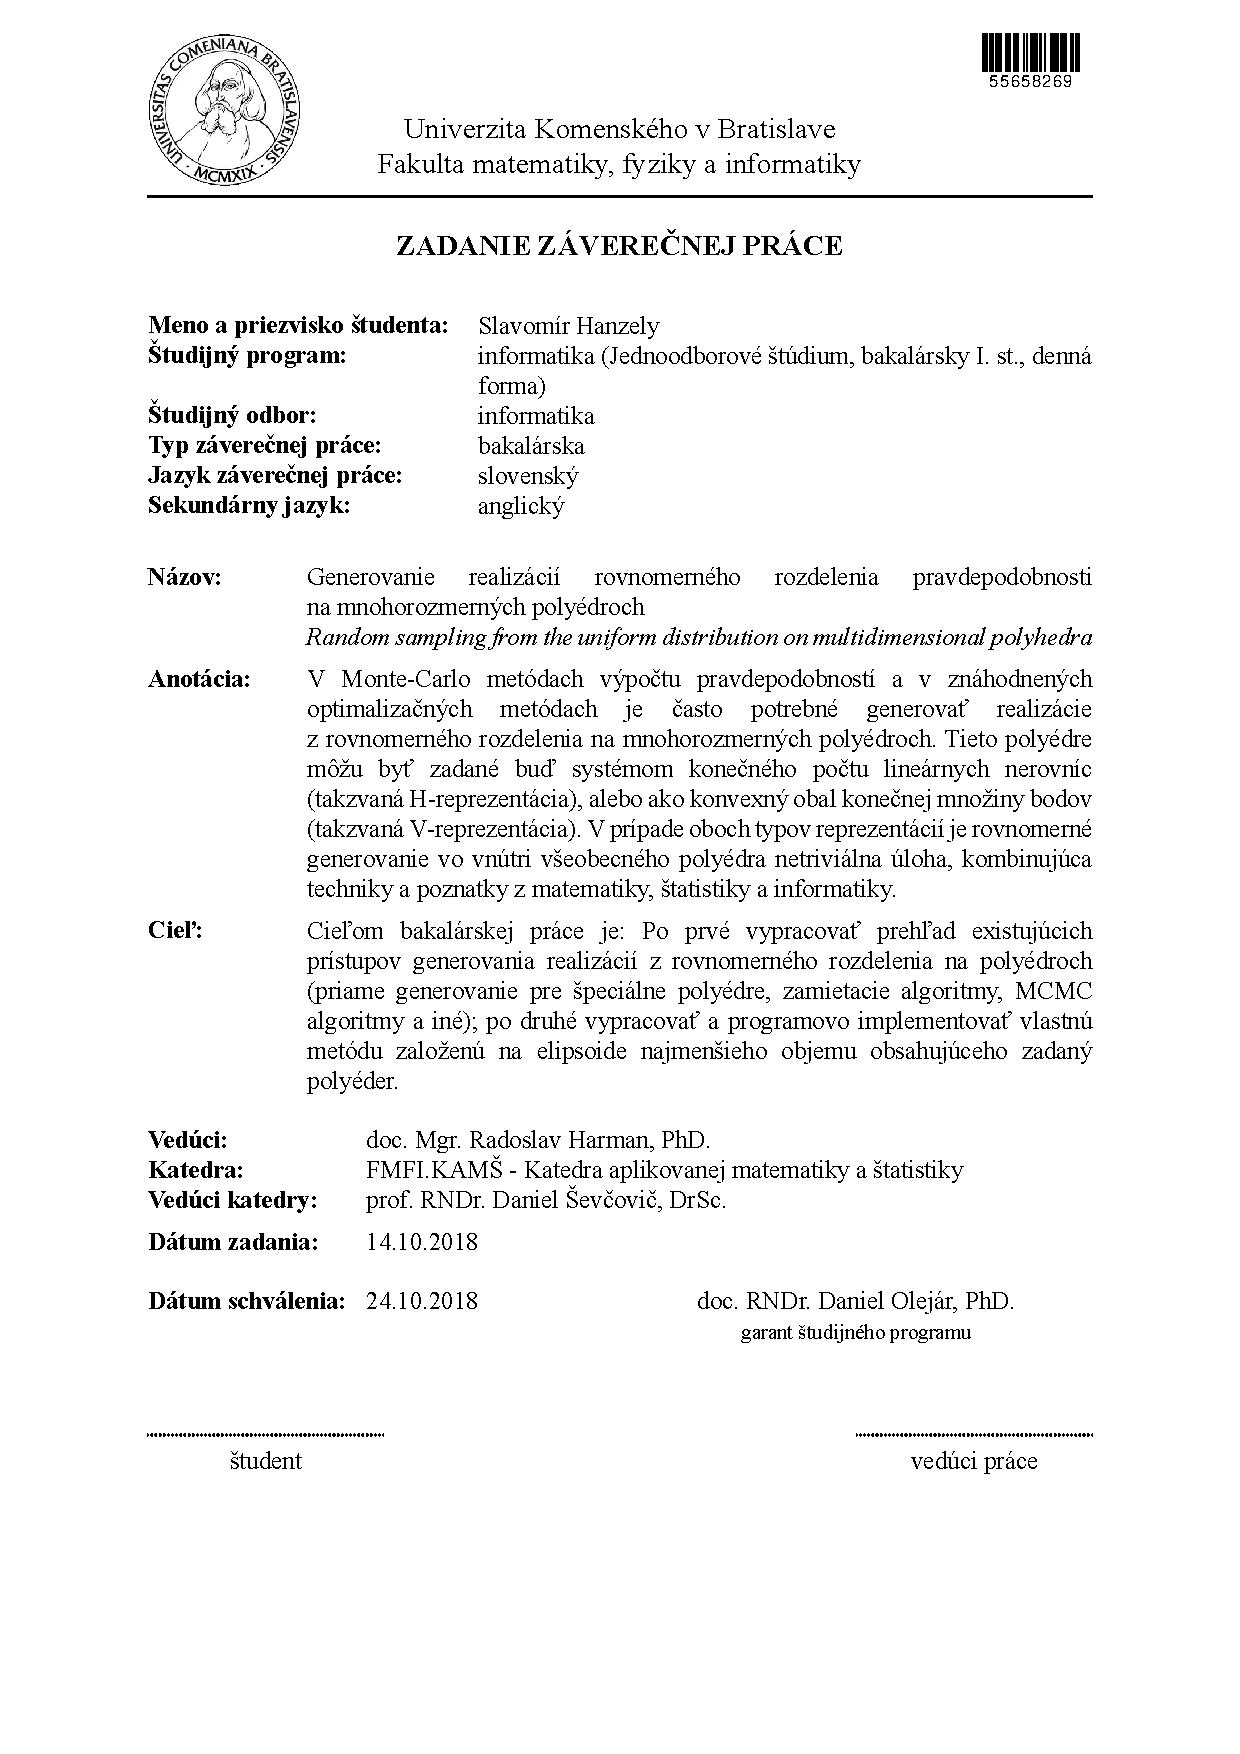
\includegraphics[width=1.1\textwidth]{images/zadanie}

% --- Koniec zadania

\frontmatter

% -------------------
%   Poďakovanie - nepovinné
% -------------------
\setcounter{page}{3}
\newpage 
~

\vfill
{\bf Poďakovanie:} 
Rád by som sa poďakoval môjmu školiteľovi doc. Mgr. Radoslavovi Harmanovi, PhD., za poskytnutie zaujímavej témy na bakalársku prácu a v neposlednom rade za podporu, cenné rady a usmernenie počas práce na nej.

% --- Koniec poďakovania

% -------------------
%   Abstrakt - Slovensky
% -------------------
\newpage 
\section*{Abstrakt}

Spravili sme prehľad existujúcich metód na generovanie bodov z rovnomerného rozdelenia na polyédri, spolu s ich praktickým porovnaním na ``náhodných'' polyédroch. 
Ako prípustné metódy sme porovnávali Gibbsov generátor a Hit--and--Run generátor z triedy Metropolis--Hastings a zamietaciu metódu pomocou nadmnožiny elipsoidu najmenšieho objemu. Ako testovacie skóre sme použili rýchlosť generovania veľkého počtu bodov v polyédri vzhľadom na rozmer priestoru. Ukázali sme, že najrýchlejší algoritmus na generovanie bodov z rovnomerného rozdelenia na polyédri je Hit--and--Run generátor. Praktické testovanie ukázalo, že prístup ku generovaniu pomocou elipsoidu najmenšieho objemu je pomalší, čo sa týka počtu realizácií za jednotku času, avšak jeho výhodou je generovanie z presného rovnomerného rozdelenia, kým algoritmy z tried Metropolis-Hastings generujú rovnomerne len limitne. Taktiež sme predstavili problém optimálneho návrhu experimentu spolu s algoritmami Vertex Exchange Method a Randomized Exchange Algorithm na jeho riešenie. Popísali sme, ako možno použiť ekvivalenciu problému D--optimálneho návrhu experimentu a elispoidu najmenšieho objemu na nájdenie elipsoidu najmenšieho objemu obaľujúceho cielený polyéder. Okrem toho sme sa venovali problému generovania náhodných polyédrov. Ukázali sme, že samotné definovanie ``náhodného polyédru'' je netriviálny problém.
% Overili sme, že so zvyšujúcim sa rozmerom priestoru očakávaný čas potrebný na vygenerovanie bodu rastie pri Hit--and--Run generátore asymptoticky lineárne, pri Gibbsovom generátore asymptoticky kvadraticky a ukázali sme, že pri zamietacej metóde s nadmnožinou elipsoidu najmenšieho objemu bude očakávaný čas rásť pravdepodobne asymptoticky exponenciálne.

\paragraph*{Kľúčové slová: Metropolis--Hastings, Hit--and--Run, Gibbs, zamietacie metódy, elipsoid najmenšieho objemu, problém optimálneho návrhu, náhodný polyéder}
% --- Koniec Abstrakt - Slovensky


% -------------------
% --- Abstrakt - Anglicky 
% -------------------
\newpage 
\section*{Abstract}

We provide a survey of existing algorithms for generating from the uniform distribution on a polyhedron with a comparison on random polyhedra. As possible algorithms, we consider a Gibbs sampler and a Hit--and--Run sampler from the Metropolis--Hastings class, as well as the rejection method using the minimum volume enclosing ellipsoid as a superset. As a score function, we use the expected generation time of a large number of points for a fixed dimension of the polyhedron. We demonstrate that the most rapid algorithm is the Hit--and--Run generator. Rejection method using the minimum volume enclosing ellipsoid is slower in practice, however, it generates points precisely from the uniform distribution in polyhedra while Metropolis--Hastings algorithms generate from distribution only converging to the uniform distribution. In addition, we introduce optimal experimental design problem with algorithms Vertex Exchange Method and Randomized Exchange Algorithm as its solvers. We show how can the equivalence of the optimal design problem and the minimum volume enclosing ellipsoid problem be used for finding minimum volume enclosing ellipsoid for given polyhedra. Moreover, we discuss random polyhedra generation. We show that just defining ``a random polyhedron'' is non--trivial problem.


\paragraph*{Keywords: Metropolis--Hastings, Hit--and--Run, Gibbs, rejection methods, minimum volume enclosing ellipsoid, optimal design problem, random polyhedra} 

% --- Koniec Abstrakt - Anglicky

% -------------------
% --- Predhovor - v informatike sa zvacsa nepouziva
% -------------------
%\newpage 
%\thispagestyle{empty}
%
%\huge{Predhovor}
%\normalsize
%\newline
%Predhovor je všeobecná informácia o práci, obsahuje hlavnú charakteristiku práce 
%a okolnosti jej vzniku. Autor zdôvodní výber témy, stručne informuje o cieľoch 
%a význame práce, spomenie domáci a zahraničný kontext, komu je práca určená, 
%použité metódy, stav poznania; autor stručne charakterizuje svoj prístup a svoje 
%hľadisko. 
%
% --- Koniec Predhovor


% -------------------
% --- Obsah
% -------------------

\newpage 

\tableofcontents

% ---  Koniec Obsahu

% -------------------
% --- Zoznamy tabuliek, obrázkov - nepovinne
% -------------------

\newpage 

%\listoffigures
%\listoftables

% ---  Koniec Zoznamov

\mainmatter


\input uvod.tex 

\input metropolis-hastings.tex

\input hit-and-run.tex

\input gibbs.tex

\input zamietacie_metody.tex

\input mvee_generation.tex

\input optimal_design.tex

\input rex.tex

\input porovnanie.tex

\input generovanie_polyedrov.tex

\input inicializacia.tex

\input zaver.tex

% -------------------
% --- Bibliografia
% -------------------
\newpage	

\backmatter

\thispagestyle{empty}
\nocite{*}
\clearpage

\bibliographystyle{plain}
\bibliography{literatura} 

%Prípadne môžete napísať literatúru priamo tu
%\begin{thebibliography}{5}
 
%\bibitem{br1} MOLINA H. G. - ULLMAN J. D. - WIDOM J., 2002, Database Systems, Upper Saddle River : Prentice-Hall, 2002, 1119 s., Pearson International edition, 0-13-098043-9

%\bibitem{br2} MOLINA H. G. - ULLMAN J. D. - WIDOM J., 2000 , Databasse System implementation, New Jersey : Prentice-Hall, 2000, 653s., ???

%\bibitem{br3} ULLMAN J. D. - WIDOM J., 1997, A First Course in Database Systems, New Jersey : Prentice-Hall, 1997, 470s., 

%\bibitem{br4} PREFUSE, 2007, The Prefuse visualization toolkit,  [online] Dostupné na internete: <http://prefuse.org/>

%\bibitem{br5} PREFUSE Forum, Sourceforge - Prefuse Forum,  [online] Dostupné na internete: <http://sourceforge.net/projects/prefuse/>

%\end{thebibliography}

%---koniec Referencii

% -------------------
%--- Prilohy---
% -------------------

%Nepovinná časť prílohy obsahuje materiály, ktoré neboli zaradené priamo  do textu. Každá príloha sa začína na novej strane.
%Zoznam príloh je súčasťou obsahu.
%
%\addcontentsline{toc}{chapter}{Appendix A}
\input appendix.tex
%
%\addcontentsline{toc}{chapter}{Appendix B}
%\input AppendixB.tex

\end{document}






